\documentclass[conference]{IEEEtran}
\usepackage[pdftex]{graphicx}
%\usepackage{epstopdf}
\graphicspath{{./png/}{./eps/}}
\DeclareGraphicsExtensions{.pdf,.png}
\usepackage[caption=false,font=footnotesize]{subfig}
\hyphenation{op-tical net-works semi-conduc-tor}
\begin{document}
\title{The design and implementation of standard-based Grid single sign-on using federated identity}

\author{\IEEEauthorblockN{Weizhong Qiang, Aleksandr Konstantinov}
\IEEEauthorblockA{Department of Physics, University of Oslo}
}

\maketitle


\begin{abstract}
When pursuing the task of making access to Grids as simple as possible, security is one of the most important challenges in production Grid infrastructures, especially when the Grid applications span multiple administrative domains as well as heterogeneous Grid middlewares. A typical example is wide scale e-Science applications which need to coordinate resources shared among a number of independent institutions with different Grid middlewares deployed on these resources. In this paper, we describe security implementation and considerations used in the upcoming version of the Advanced Resource Connector (ARC) middleware, where the heterogeneity issue has been addressed. The main goal of ARC implementation in terms of security is to let the middleware be capable of interoperating with other Grid middlewares by leveraging on standard specifications. The key aspect of the work is to enhance the current proxy certificate based authentication and single sign-on by utilizing and enhancing the standardized Web Service specifications such as Security Assertion Markup Languages (SAML), single sign-on (SSO) profile and Web Services Security in order to achieve cross-middleware authentication and single sign-on.

and more importantly, this solution can utilize the widely deployed SAML based authentication implementation in Grid systems avoiding the use of X.509 certificate on the client side.

user can get a short-lived X.509 certificate without being bothered to contact any registration authority (RA) or certificate authority (CA).

\end{abstract}

%-------------------------------------------------------------------------
\section{Introduction}
\label{sec:intro}
Grid provides the technology for wide-scale, cross-domain collaboration where users work with resources and share data which are distributed across administrative domains. This kind of collaboration is called Virtual Organization (VO)~\cite{IFoster01}. The resources that contribute to the VO can come from independent administrative domains, and even require different security approaches to access control due to usage of different underlying middlewares. The same heterogeneous situation applies to users who need to access the VO resources, because users holding one kind of a credential may need to utilize multiple resources with different security approaches. To solve the above issues, Grid middlewares should provide the following abilities:
\begin{itemize}
\item The user which participates a VO should be able to access data and resources without being required to constantly do authentication at each resource or service;
\item The VO should be able to easily manage the privileges and memberships of the users;
\item The VO together with its resources should be able to easily manage the authorization, given the condition that the resources are owned by different administrative domains.
\end{itemize}
In the current Grid community, the Grid Security Infrastructure (GSI)~\cite{IFoster98} is the de facto standard for authentication and transport level security. It builds on the Public Key Infrastructure (PKI), an architecture based on the X.509 public key certificate. GSI implements some enhancement (such as certificate delegation) based on the standard SSL/TLS protocol. Mutual authentication is required by GSI, and is the default configuration for GSI based Grid deployment.

In terms of the Virtual Organization issues mentioned earlier, GSI and some other related solutions like the Virtual Organization Management Service (VOMS) ~\cite{AlfieriR05} have partly solved them, to a different extent. The identity delegation and the X.509 proxy certificate initiated by GSI can achieve single sign-on, so that the need to re-enter the user’s pass phrase for authentication can be avoided. VOMS adopts the Attribute Certificate~\cite{RFC3821link} approach. The Attribute Certificate is signed by the VOMS server and then bound to proxy certificates by the client. Attributes include the VO membership data which is associated with the proxy certificate’s identity. Eventually the resources can make access control decisions based on parsing the VO membership attributes from the Attribute Certificate.

The VO is essentially supposed to be able to provide resource sharing capability with resources running under heterogeneous systems/middlewares. This goal can be achieved using Web Service Architecture (WSA). This way, the Web Service technology has been utilized in Grid computing middlewares, including Globus Toolkit~\cite{GTlink}, gLite~\cite{gLitelink}, as well as the Advanced Resource Connector (ARC)~\cite{ARClink}.

Unfortunately, the existing Grid security solutions such as GSI and VOMS do not apply to Web Service based applications very well due to the following reasons:
\begin{itemize}
\item The GSS API based confidential communication and identity delegation has not been adopted by Web Service implementations.
\item The Attribute Certificate has not been adopted by any aspects Web Service implementation at all.
\item Web Service implementations commonly use the Web Services Security (WS-Security)~\cite{WSSeclink}, Security Assertion Markup Languages (SAML)~\cite{SAMLlink}, and standard SSL/TLS as well as standard X.509 certificate when considering security, which make them impossible to interoperate with the GSI based Grid middlewares.
\end{itemize}

Moreover, the Grid security solutions require each user to possess a X.509 certificate. However, the process to get a certificate may take quite long time, since the requester needs to be checked and approved by the Registration Authority (RA) and only then the Certificate Authority (CA) can issue the certificate according to the approval from the RA. Meanwhile, the process to use the certificate is also not so easy for the non-IT advanced research community to deal with, since the user has to generate proxy certificates by using Grid-specific command lines, such as grid-proxy-init or voms-proxy-init. On the other hand, users could often have some more familiar local community or institutional credentials such as username/password. Enabling users to use their own community credentials instead of the X.509 certificate to access Grids is a promising solution to make the Grids more easily accessible.

The above analysis shows that in order to achieve interoperability and transparency for user to access Grid system which is established on different middlewares, we need to address the mismatch between the different security solutions from these middlewares in order to ensure the interoperability as wide as possible; it is also necessary to address the mismatch between users' daily experience and middleware's requirements in order to ensure the access as simple as possible.

The approach in the new version of ARC is to utilize the existing Web Service standards, such as SAML and WS-Security, to achieve the interoperability and accessibility without breaking existing Grid specific security protocols.

The rest of this paper is organized as follows: Section 2 presents the ARC Grid middleware, especially the architecture of the new version of ARC. Section 3 describes the solution for cross-middleware authentication and single sign-on, including implementations for bridging the mismatch in terms of authentication and single sign-on. Section 4 discusses the related research, and Section 5 presents conclusions and future work outlook.

We investigated the authentication and single sign-on issue in the scenario when a user or user's representative (acting on behalf of this user) needs to access resources across different middlewares. Our work focuses on the following five major aspects:
\begin{itemize}
	\item Integration of community authentication -- to utilize the standard-compatible community authentication mechanism from the Shibboleth~\cite{Shiblink} Identity Provider software when users authenticate against the Grid services.
	\item Short lived credentials service -- to issue the short lived X.509 certificates for users authenticated using the community authentication, in order to interoperate with the services that depend on PKI based authentication.
	\item Credential delegation service -- to process the X.509 credential delegation as a normal Web Service, in order to provide single sign-on ability.
\end{itemize}

%-------------------------------------------------------------------------
\section{ARC Grid middleware}
\label{sec:arcmiddleware}

ARC (Advanced Resource Connector) is an open source Grid middleware solution released under Apache license. ARC middleware aims at developing self-organized, fault-tolerant, non-intrusive, easy-manageable Grid middleware~\cite{MEllert07}. The current production version of ARC provides Grid services for job submission and management, resource characterization, resource aggregation and discovery, basic data management, integration of Grid security solution, and so on. This release has been deployed and used in production environment, and is one of the widely deployed Grid middlewares in Europe.

The next generation of ARC components is developed by the KnowARC project~\cite{KnowARClink}, based on the functionality and capabilities of the classic ARC middleware. It aims at implementing a Web Service oriented Grid middleware which will provide higher levels of resource and user abstraction through well-defined Web Service interface~\cite{KnowARCDesignlink} in order to provide interoperability with other service-based Grid middlewares, as well as other Web Service compatible applications.

As the key part of the implementation of new ARC middleware, there is a lightweight Web Service container called Hosting Environment Daemon (HED) which provides hosting for various services at application level, as well as a number of modules to support flexible, interoperable, and efficient communication mechanism for building SOAP based Web Services. The whole design of the HED is built around the idea of flexibility and modularity.

The architecture of the HED is illustrated in Figure \ref{fig:HED}. In general, there are few components called Message Chain Component (MCC) which are in charge of implementing different protocol levels. For instance, as shown in the example message flow, the HTTP MCC will process stream from the TLS MCC to parse the HTTP message and pass its body to the SOAP MCC, and also process the SOAP response from the SOAP MCC to generate the HTTP message for the TLS MCC.

\begin{figure}
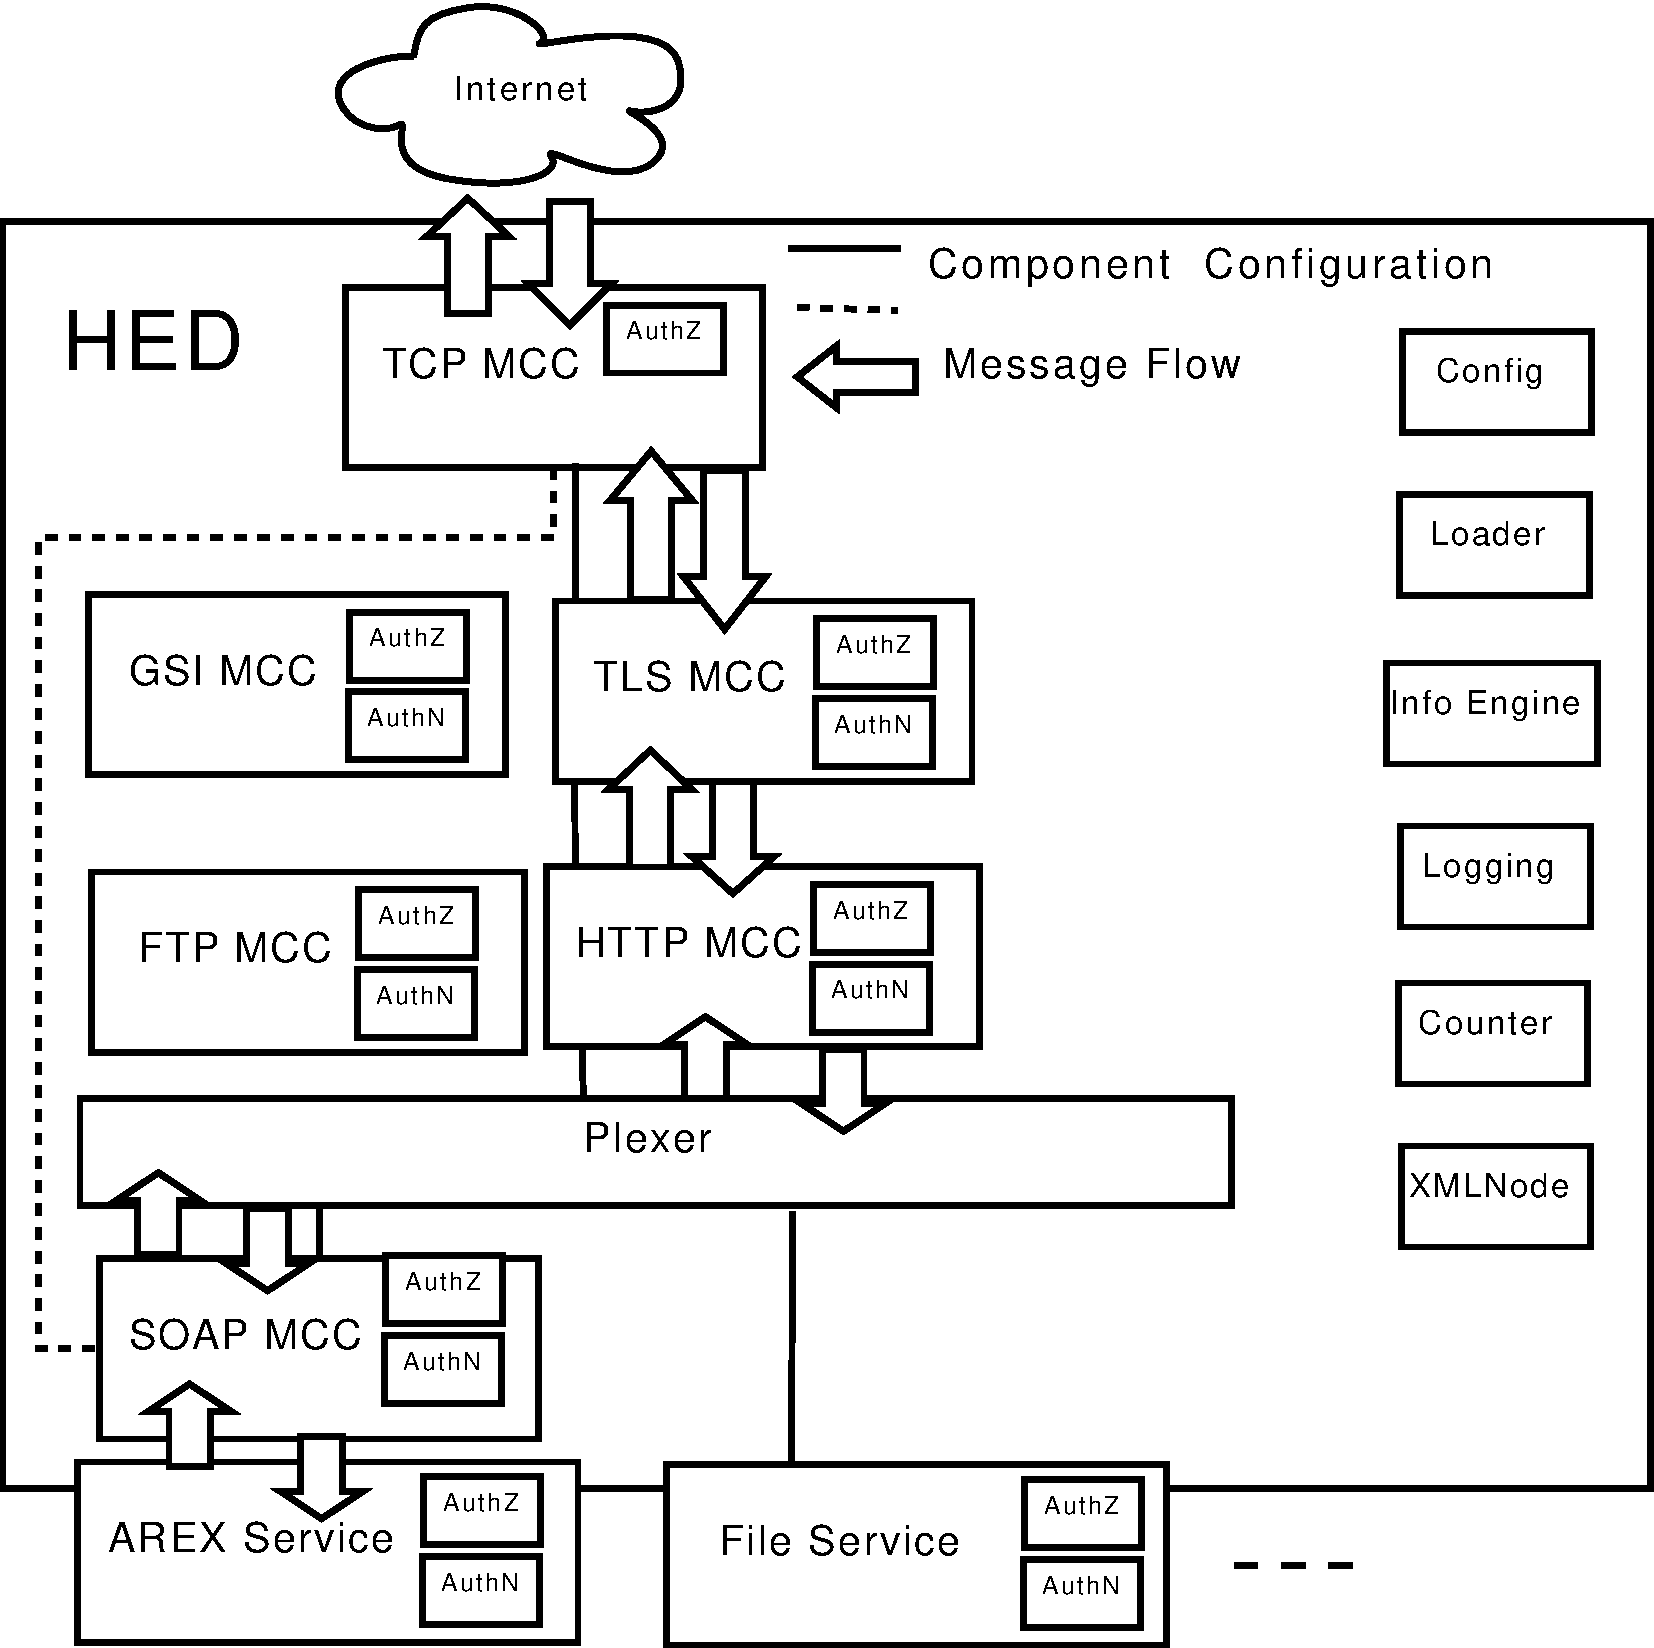
\includegraphics[width=0.9\columnwidth]{HED.pdf}
\caption{The example of Host Environment Daemon deployed with A-REX and File services}
\label{fig:HED}
\end{figure}
HED contains a framework for implementing and enforcing authentication and authorization. Each MCC or Service has a common interface for implementing various authentication and authorization functionality. Each functionality can be implemented as a pluggable and configurable component (plug-ins) called SecHandler, which is implemented as a C++ class and provides a method for processing message that travels through MCC or Service. Each MCC or Service is usually configured with two queues of SecHandler -- one for the incoming message and one for the outgoing message respectively. In Figure \ref{fig:HED}, the ``AuthZ'' and ``AuthN'' sub-modules inside MCCs and Services are examples of SecHandler.

%-------------------------------------------------------------------------
\section{Grid authentication using federated identity: Integrating SAML2SSO profile}
\label{sec:intergrationSAML2SSO}
Identity federation is an emerging technology which enables the identity information to be trustily transfered across autonomous security domains. By using identity federation, users from one domain can access another domain without the need for directly trust relationship between users and accessed domain, i.e., users can use accounts from their host domains to access external domains, and accessed domain does not need to maintain accounts for those external users. Identity federation doesn't enforce specific authentication mechanisms, so that various types of authentication can be supported between user and its host domain, and user is able to use his frequently used account/credential to accomplish authentication. Considering the Grid use cases, we see that utilizing the existing account to access Grid without being bothered to applying and manipulating a X.509 credential should be attractive for Grid users.

Shibboleth is the one of the several implementations of the identity federation, which is based on the OASIS Security Assertion Markup Language (SAML) 2.0 specifications. In terms of authentication, the Shibboleth implements SAML2.0 web browser SSO profile, which  defines two functional components, an Identity Provider and a Service Provider. The Identity Provider (IdP) is responsible for creating, maintaining, and managing user identity, while the Service Provider (SP) is responsible for controlling access to services and resources by analyzing the SAML assertions produced and issued by the IdP upon request.

In the implementation of ARC middleware, SAML2.0 web browser SSO profile is supported by implementing the functionality of service provider and web browser's user agent, and utilizing Shibboleth IdP implementation for the functionality of identity provider. The user agent functionality is for mimicing the behavior of web browser's user agent for authentication, such as the HTTP redirection and the HTTP cookie processing. The implementation of the user agent is based on the the HTTPS client interface of ARC, since the client interface of ARC can support different protocols which are incarnated by different MCCs.

\begin{figure}
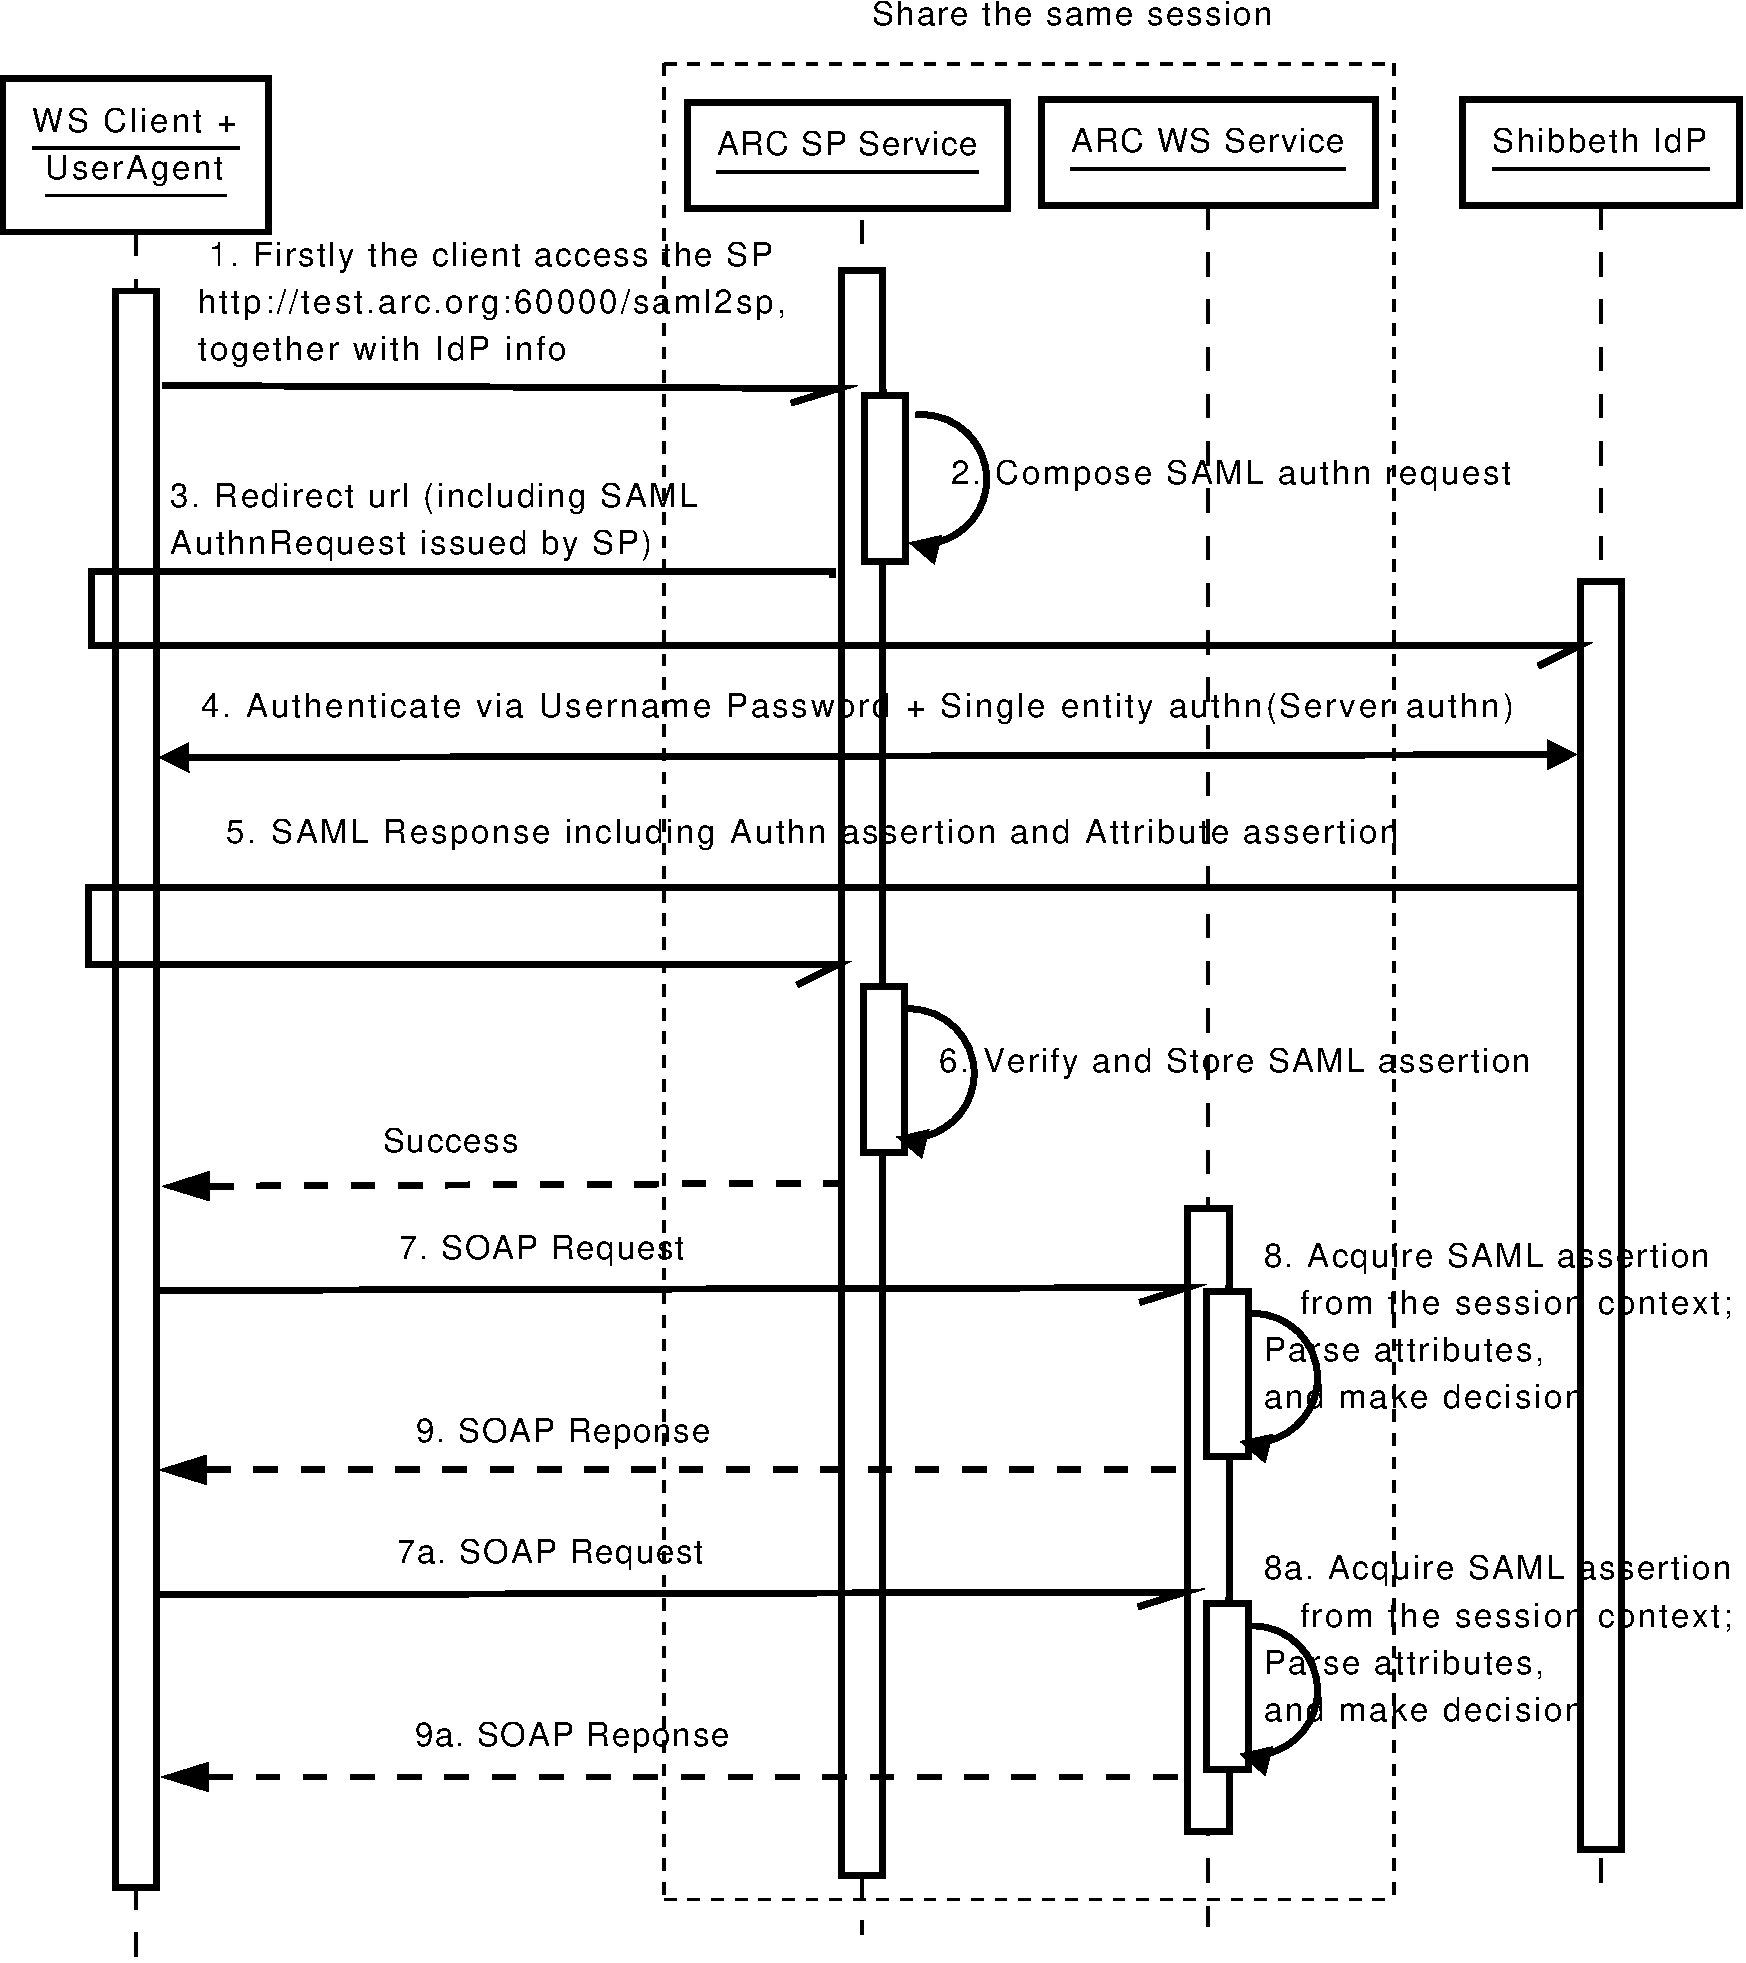
\includegraphics[width=1.0\columnwidth]{SAML2SSO_UML.pdf}
\caption{Sequence diagram of SAML2.0 SSO profile integration in SOAP invocation 
between ARC WS Client and Web Service}
\label{fig:SAML2SSOUML}
\end{figure}

Figure \ref{fig:SAML2SSOUML} shows how is SAML2.0 SSO profile integrated into the SOAP 
invocation between ARC WS Client and Web Service. Step 1 to step 5 in Figure \ref{fig:SAML2SSOUML} 
is similar to those steps depicted in Web Browser SSO profile[ref], with the differences that
we specify the way about how does the service provider determine which identity provider to use (identity
provider discovery), by enabling the client to send the IdP name to service provider; as well 
as specify the way about how does the client/user agent authenticate against service provider, 
by implementing the form-based HTTP authentication which uses username and password for authentication between 
user agent and service provider (rather than X.509 client authentication) and is compatible 
with the Username/Password login handler of Shibboleth IdP.

In step 6, the service provider (SP Service) verifies and checks the SAML response, decrypts and stores 
the SAML assertion into session/connection context. That assertion includes the AuthnStatement and 
AttributeStatement elements. From step 7 to step 9, the WS client launches the SOAP invocation via 
the same connection as the one which is used by user agent to contact SP Service, then Grid/Web Service 
checks the AuthnStatement stored in the session context to see if the AuthnStatement is valid or expired. 
If valid, service handles the SOAP request and returns the SOAP response to the WS client.

Note that in the current implementation the service requires WS client to reuse the same 
TCP connection as the one used by user agent in step 5, in order to guarantee that the validity of 
the SAML2SSO result is applicable to the SOAP invocation process. On the service side, 
the sesion reusing is accomplish by deloying the SP service and other functional Grid/Web Service(s) 
together in the same service container. 

There are a few benifits about integrating SAML2.0 SSO profile for Grid/Web service authentication. 
Firstly, the client certificate authentication can be switched off, so that users do not need 
to apply and maintain a X.509 credential. Secondly, some implementation of identity provider, such as 
Shibboleth IdP, can cache the authentication result through session management once the user
has succeeded to authenticate, and for a short period this authentication result is valid, so that 
the next time the user authenticates against IdP, the user agent can just feed IdP with the last 
successfully authenticated session's identity rather than feed IdP with username and password again. So 
the user (or the client on behalf of that user) can travel across multiple security domains with 
only providing his name and password once, which is also the characteristic of single sign-on.
Lastly, even though there are a few implementations of identity providers, most of them are 
standard-compliant, so the solution implemented in ARC middleware can interoperate with other 
identity provider implementations with minimum change.

%-------------------------------------------------------------------------
\section{Bridging federated identity and X.509 credential}
\label{sec:fedidtoX509}
Many widely used Grid middlewares are based on GSI which requires mutual X.509 authentication. 
Meanwhile, Web Service based Grid applications mostly do require client certificate authentication.  
To bridge the gap beween federated identity and X.509 credential, a short lived credential 
service (SLCS) is implemented through which a user can get a short-lived X.509 certificate only by
providing his username/password and authenticating through the SAML2SSO profile.

Also, in order to provide single sign-on capability for services that act on behalf of user to 
invoke other services, a X.509 credential delegation service is implemented, which is based on 
SOAP communication rather than the proprietary GSI communication implemented in Globus Toolkit.

\subsection{Short-lived credential service}
\label{sec:slcs}
The sequence diagram of SLCS process specializes the diagram shown in Figure \ref{fig:SAML2SSOUML}, 
with the SOAP request including X.509 request and SOAP response including X.509 response. 
In detail, the SLCS client firstly accomplishes the SAML2SSO profile, then sends 
SOAP request to the SLCS service with the X.509 request embedded. The SLCS service makes
access control decision according to the SAML assertion stored in session context, and issues 
a certificate (with 12 hours lifetime) with the SAML attributes as the X.509 certificate 
extension. The SLCS client then gets the SOAP response with the X.509 certificate embedded.

Since the lifetime of the short lived credential has a short lifetime, it is permissible to protect 
the private key by using the local file system permissions instead of encrypting it by 
using a pass-phrase. Therefore, no manual interactivity is required to uncrypted the private
key. Hence single sign-on is provided, since the user only needs to input his password when 
he starts SAML2SSO profile.

How to compose a distinguished name (DN) for the certificate is a critical issue for 
the SLCS service. We pick up the relatively identical information ``eduPersonPrincipalName'' 
(see eduPerson schema~\cite{eduSchemalink}) from SAML attributes that returned from Shibboleth
IdP, and use it to compose the DN. A typical example of the eduPersonPrincipalName 
could be alice@example.org. In such case composed DN is for example\\``/O=knowarc/OU=example.org/CN=alice''.

By using the SLCS service, the user can easily access the Grid services that requires 
X.509 credential on client side, at anywhere, simply by running the SLCS client command 
and providing his username and password.

\subsection{X.509 credential delegation service}
\label{sec:creddeleg}

\begin{figure}
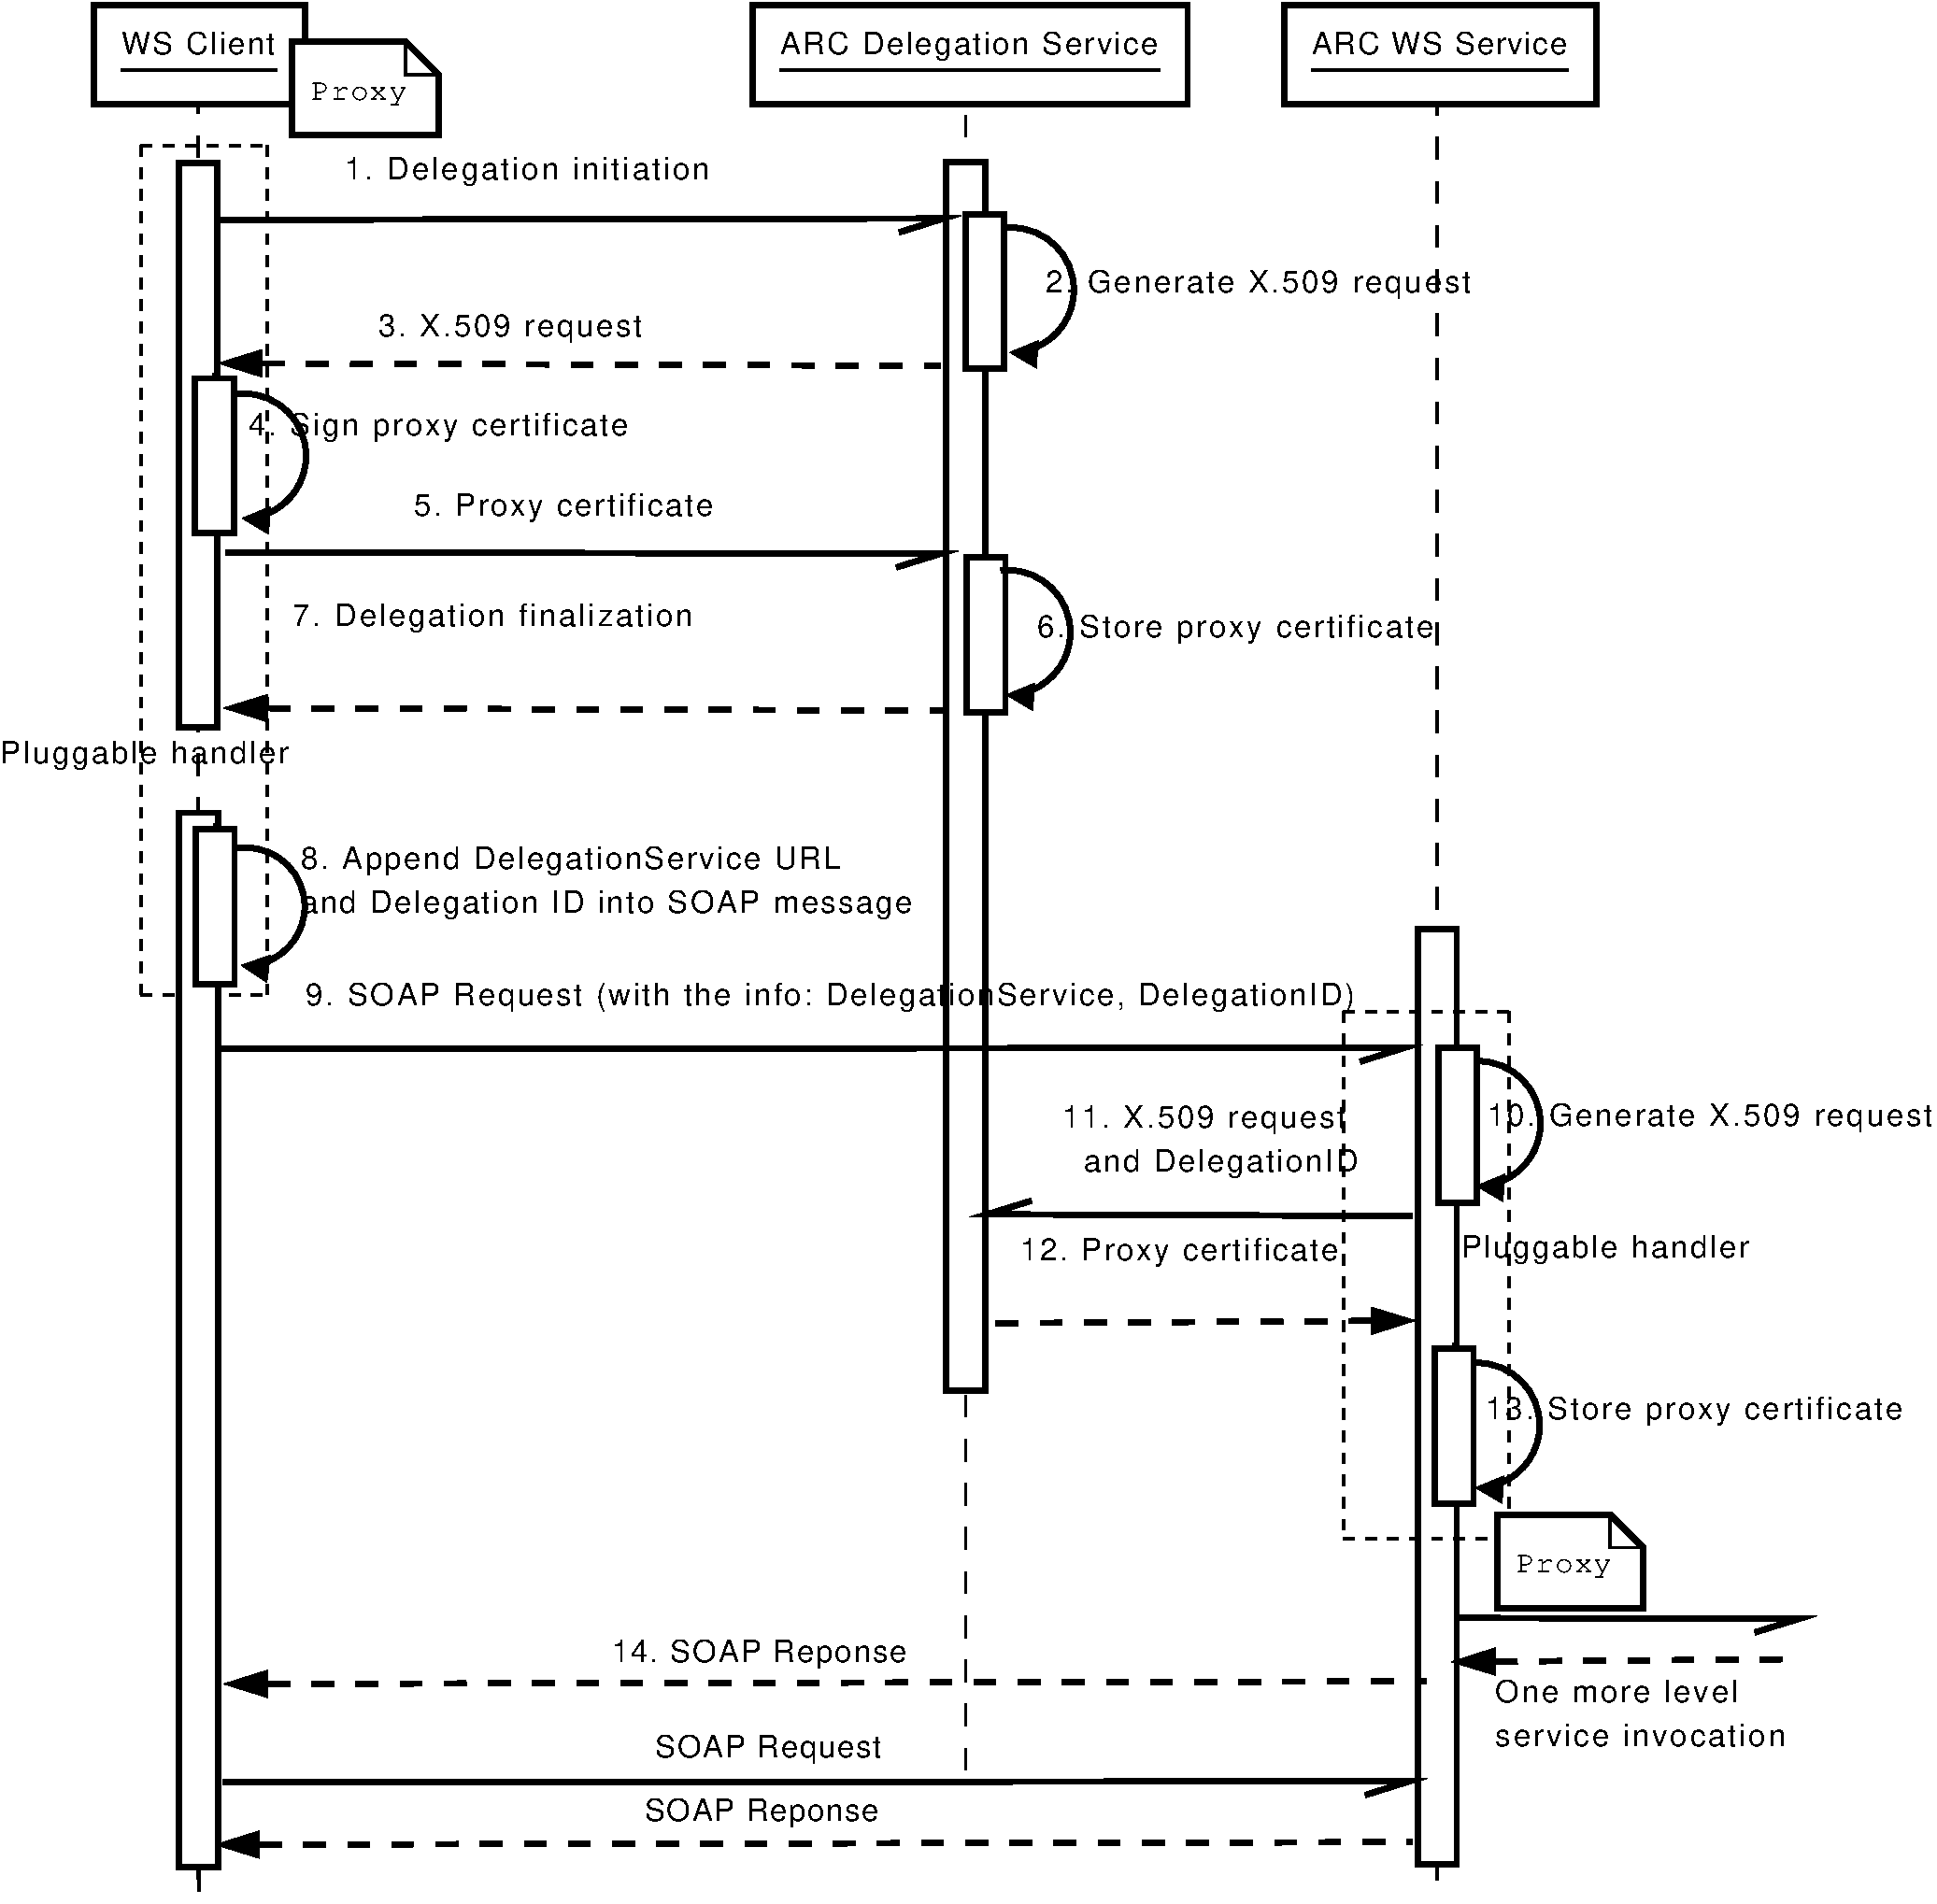
\includegraphics[width=1.0\columnwidth]{Delegation_UML.pdf}
\caption{Sequence diagram of the usage of delegation service}
\label{fig:DelegUML}
\end{figure}

The sequence diagram is shown in Figure \ref{fig:DelegUML}. Firstly, the client needs to delegate
the proxy certificate or short-lived certificate to a delegation service through step 1 to step 7.
Then this client invokes the peer Web Service by appending the delegation information (URL of delegation
service and the delegation ID corresponding to the above delegation) into the SOAP body as out-of-band 
message. The Web Service then sends a X.509 request and the delegation ID to the delegation service 
which is specified by client side, and gets back a delegated certificate which can be composed together
with the private key for a proxy certificate. The Web Service could use this proxy certificate 
to represent the user to invoke another Web Service, which either could cause one more process of 
delegation (step 1 to step 13) if another delegation service is specified, or could directly start
from step 8 if the same delegation service is specified as the one in the former delegation process.

The client only needs to delegate the certificate to delegation service one time per session, it does
not need to do delegation for subsequent SOAP invokations after the first one.

The functionality of both client and service sides are implemented as pluggable handlers which can be 
configured into the client and service configuration, so that the service or client implementation itself
does not need to be changed.

We suppose the short-lived certificate is used by client, so that the SLCS service together with
the delegation service can provide single sign-on from user's federated identity, while keeping the 
interoperability to those Grid/Web services that requires mutual authentication using certificate.

%-------------------------------------------------------------------------
\section{Performace Evaluation}
\label{sec:perfeval}
The following section evaluate the performance of the 

\subsection{Performance comparison between HED and Axis2/C}
\label{sec:perhedandaxis}
Since the implementation of HED includes an alternative SOAP implementation which is the base of 
the security related web servies described in this paper, it is useful to compare the performance 
of HED and other SOAP implementations. Although there are many SOAP implementations such as 
AxisJava, gSOAP, XSOAP4, etc., the goal of this paper is not about complete comparison between
HED and all the other SOAP implementations, so we use the Axis2/C (v1.5.0) to demostrate the performance
HED.

For the service side, we implement the simple ``echoString'' service in HED, and use the ``echoString''
service in Axis2/C. For client side, we develope a client by using API of ARC, to invoke the ``echoString''
services from Axis2/C and HED. The service invocation is just sending a short string to service, and 
getting back the same string. One test/experiment consists of a set of clients which run simultaneously. 
Each client runs for a fixed period of time, and invokes the service as many times as it can during 
the test period. Multiple clients are launched by creating multiple threads in one test.
Two values are measured: average response time and throughput. Average response time is computed
by counting the average value of the response time for each invocation. Throughput is computed
by counting the number of invocation during each second.

The two ``echoString'' services run in a test machine equipped with 3GHz Intel Pentium dual-core 
CPU and 2GB memory, Red Hat Enterprise Linux 5. The client runs in another machine equipped 
with 1.8GHz Intel Pentium CPU and 2GB memory, Ubuntu 8.10. The Axis2/C service is run using 
the httpd module on Apache Http Server version 2.2.11 instance. We keep all the configurations 
default in Apache Http Server. The client and service are configured with mutual TLS authentication.

\begin{figure}
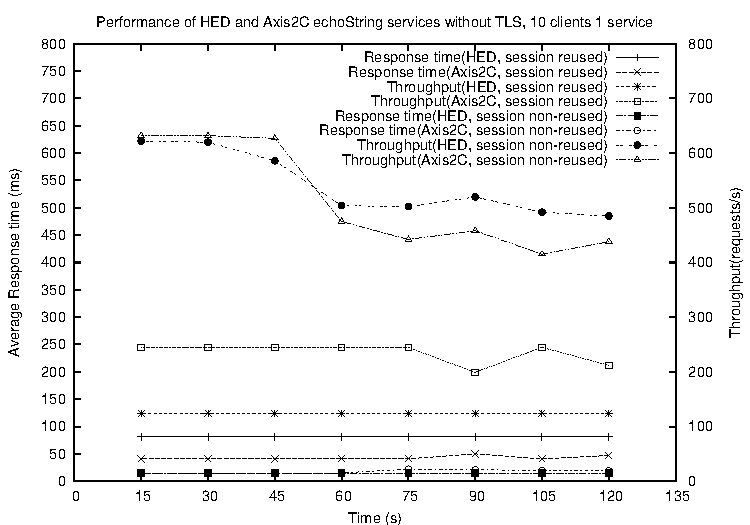
\includegraphics[width=0.9\columnwidth]{HED2Axis_thread10.pdf}
\caption{Performance results for HED and Axis2C: 1 service and 10 clients}
\label{fig:HED2Axis_thread10}
\end{figure}

\begin{figure}
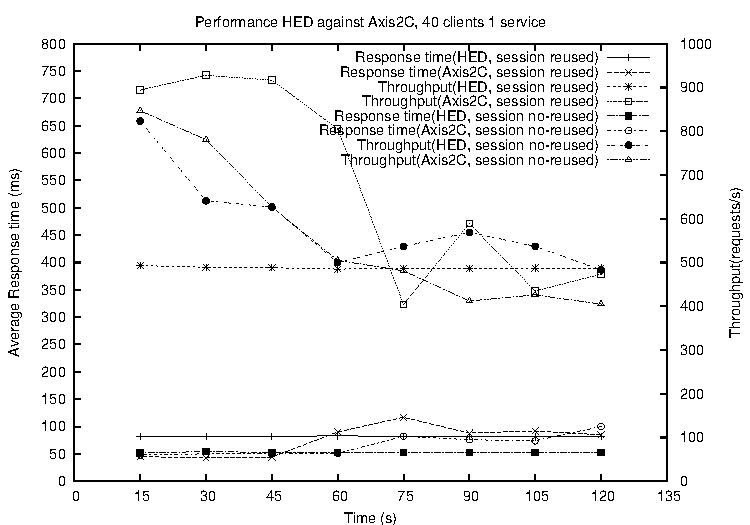
\includegraphics[width=0.9\columnwidth]{HED2Axis_thread40.pdf}
\caption{Performance results for HED and Axis2C: 1 service and 40 clients}
\label{fig:HED2Axis_thread40}
\end{figure}

Figure \ref{fig:HED2Axis_thread10} and Figure \ref{fig:HED2Axis_thread40} are the results of 
performance comparison. 
Two types of experiments are shown: session reused, session no-reused.
``Session reused'' means all of the SOAP invocations on each client share the same session 
(tcp connection); while ``Session no-reused'' means each invocation launches a new session.

For ``Session reused'' experiments, we see that the average response time in HED is about 81ms
which is twice of the value in Axis2/C, and the throughput in HED is about half of the value in Axis2/C, 
when the client number is 10. When the client number is increased to 40, the average response 
time in HED is close to the value in Axis2/C when the duration is more than 60 seconds, and the 
similar result appears for throughput. One obersavation is that, the performance results of HED is 
quite stable, with the average response time almost kept unchanged under different time points, 
as well as under different number of clients, and throughput kept unchanged under different 
time points, while increased linearly with number of clients.

For ``Session no-reused'' experiments, the average response time in HED is almost the same as
the value in Axis2/C, in both cases of client number is 10 (the value is 15ms) and 40 (the value
 is 53ms) correspondingly. On the other hand the throughput in HED is also the same as the value 
in Axis2/C, in both cases of client number is 10 and 40. One interesting obersabation is that the 
throughput is close to a fixed value (around 500 request/s) for both HED and Axis2/C in both 
cases of client number, when the duration value becomes bigger. Also, in case of client number is
40, the throughput from ``Session reused'' experiments also is close to the same fixed value.
We speculate that, with a relatively big value of client number, no matter the session is reused or
not, the throughput is becoming a fixed value which can be explained as the SOAP processing capability
of the SOAP implementation. In this case, we can believe that HED has the similar performance 
capability as Axis2/C. 

\subsection{Performance of the integration SAML2 SSO profile}
\label{sec:perfsaml2sso}
In our next experiment, we evaluate how does the integration of SAML2SSO profile impact on the 
performance of Web Service invocation. We configure a ``echoString'' service together with a SP (
Service Provider) service, and develope a client by using SAML2SSO related API of ARC, to invoke 
the ``echoString'', as well as interact with the IdP (Identity Provider). Services and client run on
the same set of machine as section \ref{sec:perhedandaxis}. Meanwhile, we deploy the Shibboleth IdP 
implementation on a machine equipped with 2.8GHz Intel Pentium CPU and 1GB memory, Red Hat Enterprise 
Linux 5.

\begin{figure}
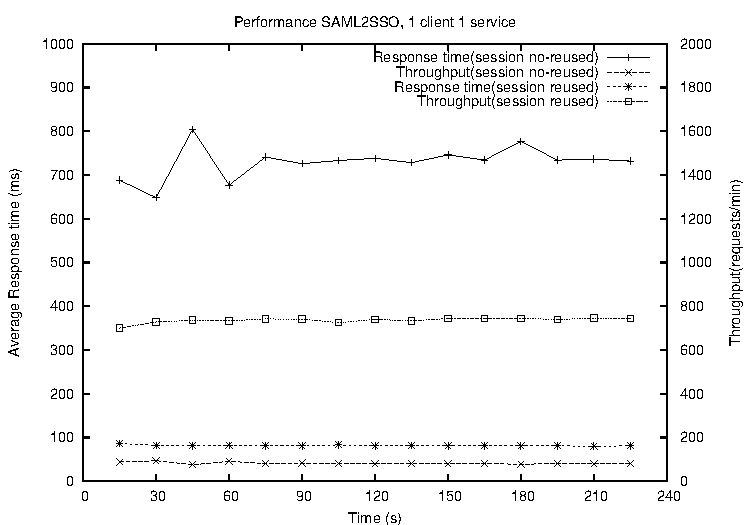
\includegraphics[width=0.9\columnwidth]{SAML2SSO_thread1.pdf}
\caption{Performance results for SAML2SSO profile: 1 service and 1 client}
\label{fig:SAML2SSO_thread1}
\end{figure}

Figure \ref{fig:SAML2SSO_thread1} depicts the average response time and throughputs for one client 
running against the service. Since the success of authentication from IdP can be regarded as 
valid for the whole session between client and service, the client with ``Session reused'' 
need to accomplish the SAML2SSO profile only once for all SOAP invocations on this client, 
while the client with ``Session no-reused'' will need to accomplish this profile once per 
SOAP invocation.

The average response time of ``Session no-reused'' experiments changes little with the execution 
duration, and the value is about 730ms; while the throughput is around 82 requests per minutes.
Considering that the average response time in case of 
``Session no-reused'' and pure SOAP invocation is around 15ms when client number is 10 (see section
\ref{sec:perhedandaxis}), not demostrated in section \ref{sec:perhedandaxis}, the same value applies 
when client number is only 1, therefore we can calculate that the consumption of time for 
SAML2SSO profile is about 98\% of the whole SOAP invocation with SAML2SSO profile integrated.
Deeper investigation about recording the time of each step of SAML2SSO profile supports the above
obersavation. In order to improve the performance of SAML2SSO profile, optimizing the process between
client and IdP is the correct direction, and probably one of the easiest way is to enhance the 
hardware configuration.

One the other hand, the average response time of ``Session reused'' experiments is about 82 ms,
which is almost as short as the value in the pure SOAP invocation experiment in \ref{sec:perhedandaxis}.
The result is resonable because the time consumption caused by only once of SAML2SSO execution on one 
client is relatively small comparing with the time consumption caused by the following hundreds 
of pure SOAP invocations.

\begin{figure}
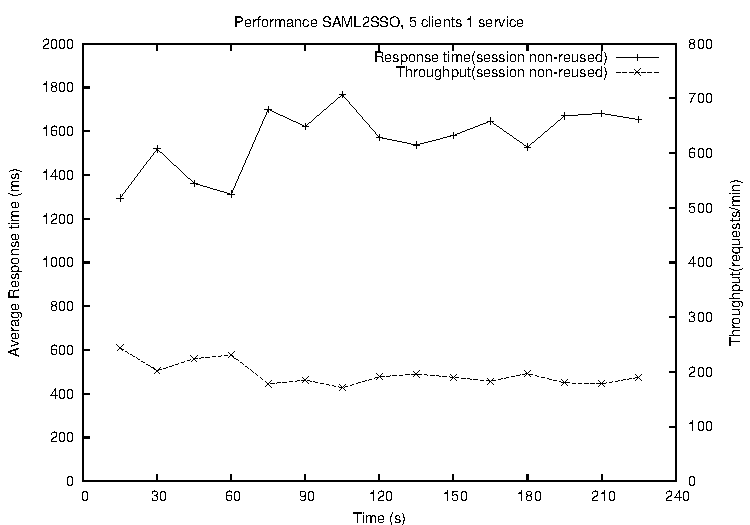
\includegraphics[width=0.9\columnwidth]{SAML2SSO_thread5.pdf}
\caption{Performance results for SAML2SSO profile: 1 service and 5 clients}
\label{fig:SAML2SSO_thread5}
\end{figure}

\begin{figure}
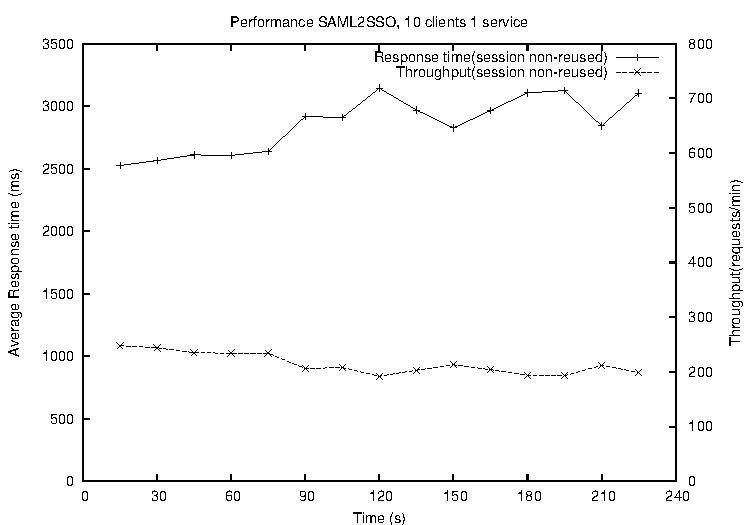
\includegraphics[width=0.9\columnwidth]{SAML2SSO_thread10.pdf}
\caption{Performance results for SAML2SSO profile: 1 service and 10 clients}
\label{fig:SAML2SSO_thread10}
\end{figure}

Figure \ref{fig:SAML2SSO_thread5} and Figure \ref{fig:SAML2SSO_thread10} depicts the average 
response time and throughputs for 5 and 10 clients running against one service simultaneously,
with the session not being reused. The throughput seems to change little with the number of 
clients increased from five to ten, with the value being abroud 200 requests per minutes;
while the average response time doubles, with the value increasing from 1.6s to 3.1s. We conclude
that in order to get acceptable response time, there should be at least less than five concurrent
clients if they need to continuously participate one SAML2SSO profile. 

However for some typical grid application scenarios, normally the client does not need 
to continuously accomplish SAML2SSO profile. For instance, a user could submit a job 
which needs a period of time (normally this period is much longer than a few seconds)
to execute, which launches an execution of SAML2SSO profile; 
afterwards, this user could query the information as well as the result about this job, which 
launches another execution of SAML2SSO profile. On the other hand, statistically, users will most
probably not access grid system in a concurrent way, rather a random way. Therefore, if we 
suppose a user could access grid once per minute, in our test environment, we can claim that 
around 200 clients randomly can be supported with acceptable performance.


\subsection{Performance of SLCS service}
\label{sec:perfslcsserv}

\begin{figure}
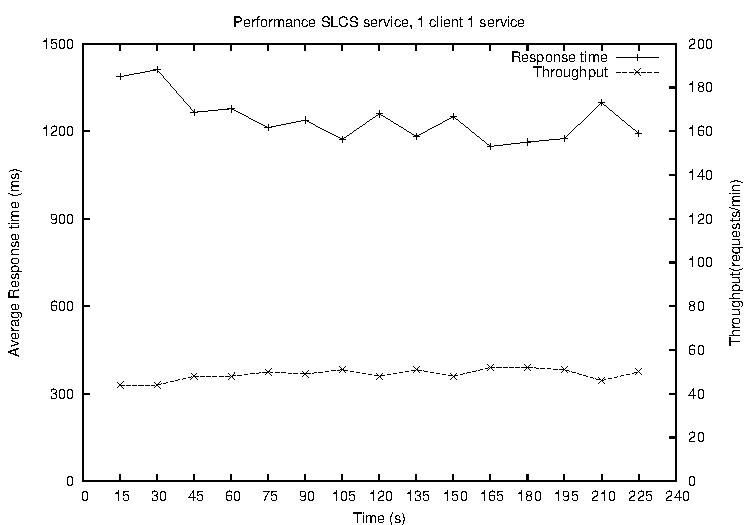
\includegraphics[width=0.9\columnwidth]{SLCS.pdf}
\caption{Performance results for SLCS service: 1 service and 1 client}
\label{fig:SLCS}
\end{figure}

Figure \ref{fig:SLCS} is the performance about the SLCS service. Since the SLCS is based on the SAML2SSO
profile, the reponse time should be the accumulation of time consumption about the SAML2SSO processing 
and the SLCS processing. In this experiment, SLCS service and client run on the same set of machine 
as section \ref{sec:perhedandaxis}. This figure shows that the average response time changes little with
the execution time with the value being around 1.3s which is nearly double as the value (730ms) of one client 
experiment about ``echoString'' service invocation with SAML2SSO integrated. Not demostrated in 
Figure \ref{fig:SLCS}, the more consumption of time is caused by the creating of X.509 request on the
 client side, which takes about roughly 310ms in average, as well as by the signing of X.509 certificate 
on the SLCS service side, which takes roughly 33ms in average, together with the time consumption for 
communication.

Even though the average response time of SLCS service is not very short, considering the short-lived 
credential has a relatively long lifetime (12 hours by default) and therefore client only needs to invoke
SLCS service once per 12 hours, the performance is completely acceptable. Also considering the time 
consumption for the creation of X.509 request (1024-bit RSA key pair generation) is on the client side,
we speculate the SLCS service side will not be affected much by the time-consuming key pair generation, and
therefore its performance resemble the performance of SAML2SSO profile in section \ref{sec:perfsaml2sso}.

\subsection{Performance of delegation service}
\label{sec:perfdelegserv}

In the last experiment, we evaluate how does the usage of delegation service impact on the 
performance of Web Service invocation. We deployed a ``echoString'' service plugged with delegation
security handler on a machine equipped with 2.80GHz Intel Pentium CPU and 1GB memory, Red Hat 
Enterprise Linux 5, and also configure a client together with delegation security handler plugged 
on a machine equipped with 1.8GHz Intel Pentium CPU and 2GB memory, Ubuntu 8.10. Aside from 
``echoString'' service and client, a delegation service is deployed on a machine equipped with 
3GHz Intel Pentium dual-core CPU and 2GB memory, Red Hat Enterprise Linux 5.

\begin{figure}
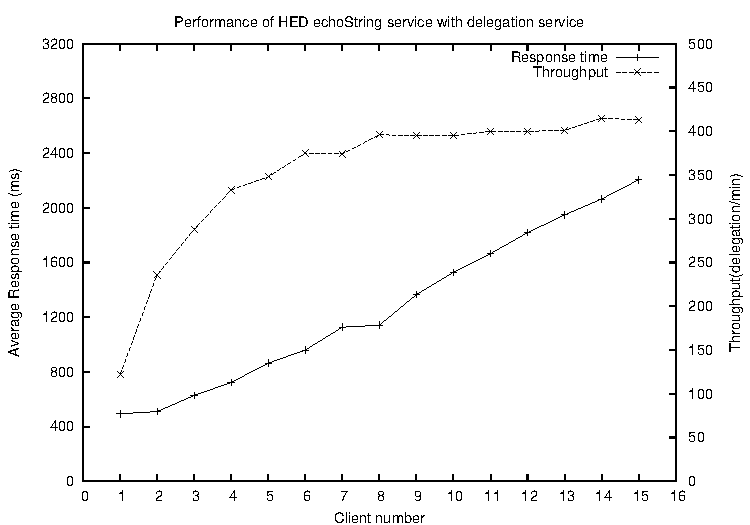
\includegraphics[width=0.9\columnwidth]{Delegation_thread_to_perf.pdf}
\caption{Performance results of delegation service: from 1 client to 15 clients}
\label{fig:Deleg}
\end{figure}

Initial experiments which are not demonstrated in this paper show that both the response time and
throughput almost do not change with the time. Therefore, we measure the performance as the function 
of the client numbers from 1 to 15. Figure \ref{fig:Deleg} is performance results. We see that 
the response time increases in a linear manner against client numbers; and the throughput gradually 
increases, and stops increasing and almost keeps unchanged when the client number is bigger than eight.
We conclude that if the client number is bigger than eight, in our test environment, there is no 
throughput benefit can be achieved by adding clients.


%-------------------------------------------------------------------------
\section{Related Work}
\label{sec:relatedwork}
Similar work that integrates Shibboleth and Grid middleware does exist. GridShib~\cite{VWelch05,TBarton06} uses Shibboleth to get entity's attribute for the authorization of services developed in Globus Tookit. Unlike the work described in this paper, the GridShib does not use Shibboleth's native login handlers for authentication to Shibboleth IdP, instead, a new login handler specific for X.509 based authentication is developed for the Shibboleth IdP, and a credential service is developed for acting as an online-CA, authenticating the user, and issuing short-lived X.509 credential. Moreover, this paper provides a single sign-on solution for the user with community credentials authenticating to Grid services by directly using SAML2.0 SSO profile.

SWITCH (The Swiss Education and Research Network) short-lived credential service (SLCS)~\cite{switchslcslink} provides a SLCS service and a client. The advantage of our work comparing to the SWTCH's solution is that the SLCS service and client are based on Web Services, so that they can be implemented in any Web Service container while keeping interoperability.

In terms of delegation, apart from the credential delegation mechanism of GSI~\cite{IFoster98,VWelch04}, several authors~\cite{MAhsant04} propose a delegation protocol based on the WS-Trust~\cite{WSTrustlink} in order to provide a standard and interoperable protocol for the delegation in Grids. WS-Trust will also be adopted by the ARC middleware to express the specifications required to define delegation protocol in a standard way. Gridsite project implements a X.509 credential delegation solution~\cite{GridSitelink} based on the Web Service, with which ARC delegation client can be made easily interoperable.

%-------------------------------------------------------------------------
\section{Conclusion And Future Work}
\label{sec:conclusion}
In this paper we presented the solution built into the ARC Grid middleware, aiming towards the cross-middle-ware authentication and single sign-on. The goal of our work is to develop an interoperable and accessible single sign-on solution to be used for a VO scenario in production Grids, where users can easily authenticate against the Grids with any of their credentials (not only X.509) from anywhere, and move inside Grid middleware infrastructure and even across heterogeneous Grids  boundaries, without re-authentication within a reasonable period. In order to do so, we implemented some standards based Web Services (including the SLCS service, the X.509 credential delegation service, and the SAML Token delegation service), as well as the user agent and the Service Provider in the context of the SAML2 SSO profile.

It must be noted that due to the standard specifications utilized (SAML and WS-Security) which are independent from any particular middleware, the WS clients and Web/Grid Services developed within the ARC middleware can interoperate with WS clients and Web/Grid Services developed as part of some other middlewares in a standardized way.

Though only authentication issue is discussed in this paper, as the future work, we will implement a solution for cross-middleware attribute-based authorization by using the standard specifications such as SAML.



% An example of a floating figure using the graphicx package.
% Note that \label must occur AFTER (or within) \caption.
% For figures, \caption should occur after the \includegraphics.
% Note that IEEEtran v1.7 and later has special internal code that
% is designed to preserve the operation of \label within \caption
% even when the captionsoff option is in effect. However, because
% of issues like this, it may be the safest practice to put all your
% \label just after \caption rather than within \caption{}.
%
% Reminder: the "draftcls" or "draftclsnofoot", not "draft", class
% option should be used if it is desired that the figures are to be
% displayed while in draft mode.
%
%\begin{figure}[!t]
%\centering
%\includegraphics[width=2.5in]{myfigure}
% where an .eps filename suffix will be assumed under latex, 
% and a .pdf suffix will be assumed for pdflatex; or what has been declared
% via \DeclareGraphicsExtensions.
%\caption{Simulation Results}
%\label{fig_sim}
%\end{figure}

% Note that IEEE typically puts floats only at the top, even when this
% results in a large percentage of a column being occupied by floats.


% An example of a double column floating figure using two subfigures.
% (The subfig.sty package must be loaded for this to work.)
% The subfigure \label commands are set within each subfloat command, the
% \label for the overall figure must come after \caption.
% \hfil must be used as a separator to get equal spacing.
% The subfigure.sty package works much the same way, except \subfigure is
% used instead of \subfloat.
%
%\begin{figure*}[!t]
%\centerline{\subfloat[Case I]\includegraphics[width=2.5in]{subfigcase1}%
%\label{fig_first_case}}
%\hfil
%\subfloat[Case II]{\includegraphics[width=2.5in]{subfigcase2}%
%\label{fig_second_case}}}
%\caption{Simulation results}
%\label{fig_sim}
%\end{figure*}
%
% Note that often IEEE papers with subfigures do not employ subfigure
% captions (using the optional argument to \subfloat), but instead will
% reference/describe all of them (a), (b), etc., within the main caption.


% An example of a floating table. Note that, for IEEE style tables, the 
% \caption command should come BEFORE the table. Table text will default to
% \footnotesize as IEEE normally uses this smaller font for tables.
% The \label must come after \caption as always.
%
%\begin{table}[!t]
%% increase table row spacing, adjust to taste
%\renewcommand{\arraystretch}{1.3}
% if using array.sty, it might be a good idea to tweak the value of
% \extrarowheight as needed to properly center the text within the cells
%\caption{An Example of a Table}
%\label{table_example}
%\centering
%% Some packages, such as MDW tools, offer better commands for making tables
%% than the plain LaTeX2e tabular which is used here.
%\begin{tabular}{|c||c|}
%\hline
%One & Two\\
%\hline
%Three & Four\\
%\hline
%\end{tabular}
%\end{table}


\section*{Acknowledgment}


The authors would like to thank...





% trigger a \newpage just before the given reference
% number - used to balance the columns on the last page
% adjust value as needed - may need to be readjusted if
% the document is modified later
%\IEEEtriggeratref{8}
% The "triggered" command can be changed if desired:
%\IEEEtriggercmd{\enlargethispage{-5in}}

% references section


%\bibliographystyle{IEEEtran}

\begin{thebibliography}{1}

\bibitem{IFoster01}
I. Foster, C. Kesselman, S. Tuecke. The anatomy of the Grid: Enabling scalable virtual organizations, International Journal of Supercomputer Applications, 15(3), 200-222 (2001)

\bibitem{IFoster98}
I. Foster, C. Kesselman, G. Tsudik, and S. Tuecke, A Security Architecture for Computational Grids, ACM Conference on Computers and Security, 1998, 83-91.

\bibitem{AlfieriR05}
R. Alfieri, R. Cecchini, V. Ciaschini, L. dell’Agnello, A. Frohner, K. Lorentey, and F. Spataro. From gridmap-file to voms: managing authorization in a Grid environment. Future Generation Comp. Syst., 21(4), 549-558 (2005)

\bibitem{RFC3821link}
RFC 3821- An Internet Attribute Certificate Profile for Authorization. http://www.faqs.org/rfcs/rfc3281.html

\bibitem{GTlink}
Globus Toolkit. http://www.globus.org/toolkit/

\bibitem{gLitelink}
gLite: lightweight middleware for Grid computing. http://glite.web.cern.ch

\bibitem{ARClink}
Advanced Resource Connector. http://www.nordugrid.org/middleware/

\bibitem{WSSeclink}
OASIS Web Services Security. www.oasis-open.org/committees/wss/

\bibitem{SAMLlink}
OASIS Security Assertion Markup Languages (SAML). www.oasis-open.org/committees/security/

\bibitem{MEllert07}
M. Ellert et al. Advanced resource connector middleware for lightweight computational grids, Future Generation computer systems, 23(2), 219-240 (2007)

\bibitem{KnowARClink}
KnowARC project.  https://www.knowarc.eu/

\bibitem{KnowARCDesignlink}
Design document of new version ARC. https://www.knowarc.eu/documents/Knowarc\_D1.1-1\_07.pdf

\bibitem{Shiblink}
The Shibboleth Project. http://shibboleth.internet2.edu/

\bibitem{eduSchemalink}
eduPerson and eduOrg Object shema. http://middleware.internet2.edu/eduperson/

\bibitem{VWelch05}
V. Welch, T. Barton, K. Keahey and F. Siebenlist. Attributes, Anonymity, and Access: Shibboleth and Globus Integration to Facilitate Grid Collaboration. 4th Annual PKI R\&D Workshop, 2005.

\bibitem{TBarton06}
T. Barton et al. Identity Federation and Attribute-based Authorization through the Globus Toolkit, Shibboleth, Gridshib, and MyProxy. 5th Annual PKI R\&D Workshop, 2006.

\bibitem{switchslcslink}
SWITCH Short Lived Credential Service. http://www.switch.ch/Grid/slcs/

\bibitem{VWelch04}
V. Welch et al. X.509 proxy certificate for dynamic delegation, Proceeding of the 3rd Annual KI R\&D Workshop, 2004.

\bibitem{MAhsant04}
M. Ahsant, J. Basney, and O. Mulmo. Grid Delegation Protocol, UK Workshop on Grid Security Experiences, Oxford. 2004.

\bibitem{WSTrustlink}
OASIS WS-Trust specification. http://docs.oasis-open.org/ws-sx/ws-trust/200512

\bibitem{GridSitelink}
Gridsite delegation service. http://www.gridsite.org/wiki/Delegation\_protocol

\end{thebibliography}




\end{document}


